\chapter{Conclusions}
\label{chap:conclusions}

\section{Conclusion}
%How can a UABS network be optimized to minimize global exposure or overall power consumption? 
All conclusions are based on the default configuration as described in table \ref{table:defaultconf} unless mentioned otherwise.
Literature showed that a network can be optimized towards either the power consumption of the entire network 
or the electromagnetic exposure of the average user using a fitness function. This is because the power required to activate a new 
base station is much higher then for expanding its range \cite{J1}.
The fitness function was originally applied for fixed transmission towers but can also be used 
for \gls{UABS}s as this research shows.
However, the fitness function should be used with care considering that \gls{UABS}s can be placed anywhere as opposed to 
the transmission towers from \cite{J1} who have a predetermined position.  
In an exposure optimized network, this causes a lot of users to get a \gls{UABS} all by themselves because this is the best approach to minimize exposure.
A power consumption optimized network on the other hand will try to limit the number of drones 
in order to save energy. So as a rule of thumb: an exposure optimized network will result in a lot of low powered devices (increasing the overall power consumption)
while a power consumption optimized network results in a few high powered devices (increasing the exposure of the average user).
If the goal is to remain in the air for a longer period of time, an exposure optimized network is recommended because the power consumption of 
an individual \gls{UABS} is lower.
On the other hand, a power consumption optimized network is cheaper because less drones are involved.
Moreover, the results show that the electromagnetic radiation in a power consumption optimized network (with high powered \gls{UABS}s)
is far below the thresholds enforced by the Flemish government.

The user's main sources of exposure are the user's own device and the \gls{UABS} who is serving him, followed by all
other \gls{UABS}s in the network. 
When the population increases, also the exposure from other people's \gls{UE} increases. However, the electromagnetic
 exposure from these devices can be ignored compared to the much higher electromagnetic exposure from the other sources. 
A bigger population also causes an increase in number of drones. So when the population grows, the exposure of the 
user increases mainly because of a growing exposure from other \gls{UABS}s that are not serving the user.
An exposure optimized network will limit the total exposure mainly by trying to reduce the exposure from other \gls{UABS}s.

%1)	How does the network behave differently after the introduction of a realistic antenna?
A directional microstrip patch antenna is introduced because it gives several advantages compared to omnidirectional antennae.
Directional antennae are able to focus their energy there where it is needed, namely towards the ground. Microstrip patch antennae 
further benefit from their thin and lightweight design. The performance 
of this directional microstrip patch antenna has been compared to a 
fictional \gls{isotropicradiator}.
This \gls{isotropicradiator} has higher exposure and coverage for less power compared to realistic antennae like microstrip patch antennae
because of the absence of attenuation and can hypothetically be compared to an antenna with a very big aperture angle.
This type of antenna can achieve the same coverage with less
resources like power and number of drones. 
A microstrip patch antenna with a more limited aperture angle of \ang{90} requires more resources but 
causes less sideways radiation. So the exposure from other \gls{UABS}s will be way less.

\begin{figure}[hb!]
  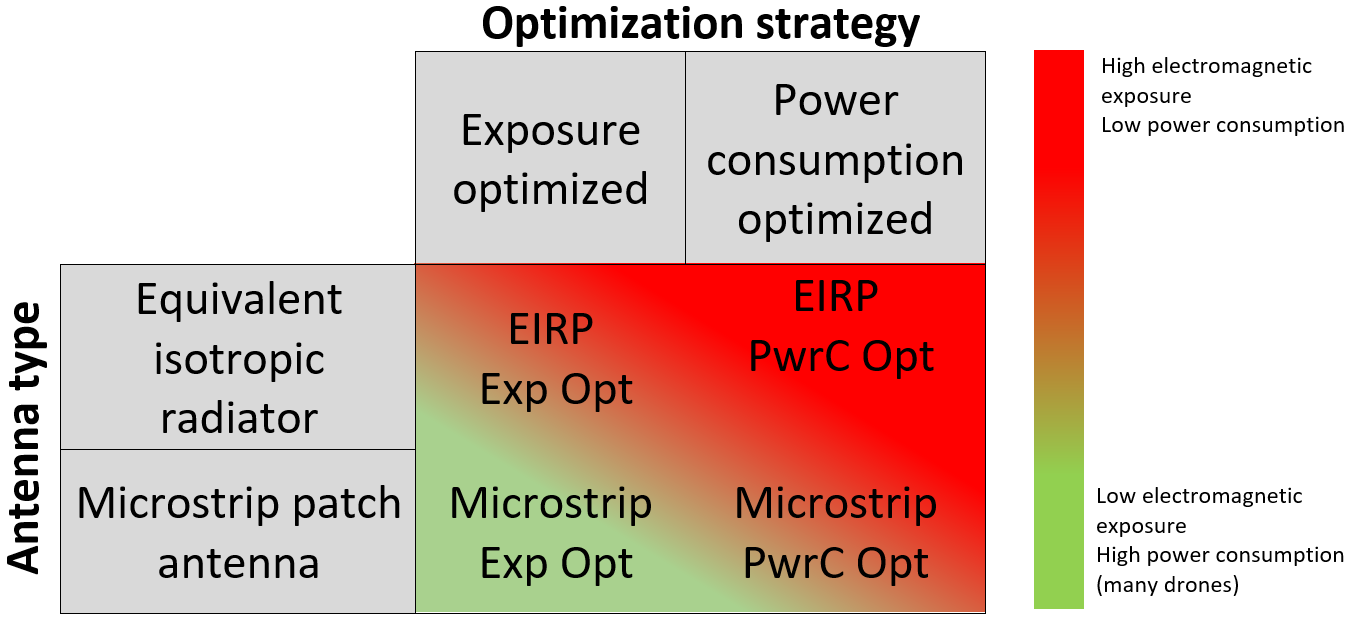
\includegraphics[width=\textwidth]{../images/fourCasesMatrixSol.png}
  \caption{Matrix with the four possible configurations, colour-coded based on the results.}
  \label{fig:resultIllustration}
\end{figure}

Remarkable is that an \gls{EIRP} exposure optimized network behaves very similar to a microstrip power consumption optimized network as shown 
in figure \ref{fig:resultIllustration}.
This results in the best of both worlds. 
The microstrip patch antenna will generate less electromagnetic radiation by design and
 the power consumption optimization reduces the number of required drones and power. A microstrip patch antenna with an aperture 
 angle of \ang{90} is considered as a good solution but if budget is more limited, an antenna with a larger aperture angle 
 would further reduce cost without interfering with the Flemish legislation regarding electromagnetic exposure.

The electromagnetic radiation of an exposure optimized network increases with higher flying altitudes. This increase is mainly caused by the user's 
own device and \gls{UABS}s who are serving other users. Around 80 metres, the exposure from the  user's device surpasses the exposure from the serving \gls{UABS}.
On the other hand, a power consumption optimized network shows a more concave relationship with the lowest exposure measured around 70 to 80 metres.
Further, the results also show that the number of required drones decreases when the flying height becomes larger; a conclusion that was also made in \cite{J2}.
 When also considering the results from \cite{U1} where a flying altitude of  
80 metres is suggested for an optimal access and backhaul connectivity, a flying height 
of 80 metres is also here proposed for the city centre of Ghent.

In short, a power consumption optimized network is proposed with a fixed flying height of 80 metres. A microstrip patch 
antenna with a sufficiently large aperture angle is a good starting point.  However, different antenna array configurations still have to 
be investigated.

\section{Future work}

The chosen microstrip patch antenna is solely based on literature and performing an excessive research to various 
types of radiation patterns is outside the scope of this master dissertation. It is expected that the radiation can 
further be improved by using microstrip patch antennae in more complex array-configurations.

Also, the tool makes use of an \gls{exact algorithm}. Despite the fact that several  
tactics have been introduced to improve performance, large populations still cause long runtimes. It might be useful 
to reduce the quality of the result in order to improve performance. Mozafari et al. discusses in \cite{U3} several 
other approaches besides \gls{exact algorithm}s like heuristic methods, machine learning and so on.